
\chapter{Mapping}

\renewcommand{\epigraphsize}{\footnotesize}
\epigraph{`Would you tell me, please, which way I ought to go from here?'

  `That depends a good deal on where you want to get to,' said the Cat.

  `I don't much care where--' said Alice.

  `Then it doesn't matter which way you go,' said the Cat. }{Alice's Adventures
  in Wonderland

  by Lewis Carroll}
  
Mapping is not a pre-defined concept, there are different ways to think about
mapping, all depends on one's need. The unifying idea is a method to fuse and
represent geometric information about a given environment. Nevertheless, the
meaning of how to represent which information is a consequence of the
application. Here, in this thesis, the objective is to have human-understandable
map yet with a probabilistic interpretation of a 3D environment. 

\section{Map Representation}
\label{s:map_rep}
Classically maps are binary functions over the space. The binary choices of
function's range stand for fullness or emptiness of a point.
Mapping (occupancy maps) is to construct a probability distribution over the set
$\mathcal{M}_d$ of all maps~\cite{thrunprob} on a given dimension $d$, i.e.
$\mathcal{M}_d=\{\coord{m}~|~\coord{m}:\mathbb{R}^d\to\{0,1\}\}$. The
cardinality of such a set $|\mathcal{M}_d|$ is too big\footnote{Side note: the
actual mathematical cardinality is $\beth_2=\mathbf{2}^\mathfrak{c}$ the
cardinality the power set of the continuum, where $\mathfrak{c}$ is the
cardinality of the continuum } to be tractable by exhaustion even considering
computational discretization (finite precision),i.e. by individually
assigning probabilities to each map.

Three approaches to this problem are presented here. One option is to consider
conditional independence of spatial points and discretize the space even
further, until it becomes tractable.
Another is to renounce the idea of binary maps and consider maps to be a collection of predefined
objects. And lastly, keep the concept of binary maps, but to consider some
restriction on the space of functions from which the map $\coord{m}$ is drawn.

Despite their differences, all approaches describe marginal probabilities, which
are functions over $\mathbb{R}^d$, instead of the probability for an actual map
$\coord{m}$, whose domain is $\mathcal{M}_d$.
Thus, for binary maps, the important quantity is
$\Pr(\coord{m}(x^\ast)=1)$\footnote{The $1$ here is completely arbitrary, it
might as well be $0$, as both probabilities are complementary.}, where $x^\ast
\in \mathbb{R}^d$, and not $\Pr(\coord{m}^\ast=m_i)$, where $m_i \in
\mathcal{M}_d$. When considering maps as collection of objects, the conditional
probability is $\Pr(\mathfrak{s}(\mathbf{l}_n)=\mathfrak{s}_i)$, where
$\mathfrak{s}(\parm)$ is the defining properties of an object $\mathbf{l}_n$,
e.g. $\mathbf{l}_n$ belongs to the set of segments and $\mathfrak{s}(\mathbf{l}_n)$
gives its pair of endpoints.

\subsection{Discrete Map}

Discrete maps are also denominated \textit{grid maps} because when discretizing
each axis of a $\mathbb{R}^d$ space the result is necessarily a grid. Originally
developed for 2D maps~\cite{thrunprob}, they were later extended to 3D maps
in different ways.

\subsubsection{3D grids}
\label{sss:3dgrid}
The first obvious extension was a 3D grid of cubes by discretizing a range
of each direction on $N$ elements. Reasoning that each cube still full
or empty, the set of possible maps on a $N_1\times N_2\times
N_3$ grid $\mathbf{D}$ is
$\bar{\mathcal{M}}_d=\{\coord{m}~|~\coord{m}:\mathbf{D}\to\{0,1\}\}$. The
cardinality of $|\bar{\mathcal{M}}_d|=2^{N_1\cdot N_2\cdot
N_3}$ is too big to store the probability of every element. 

The simplifying assumption for 3D grid is the conditional independence of grid
elements $\coord{m}(d_i)$ and $\coord{m}(d_j)$ on the sensors measurements
$\mathbf{z}_n$, for $d_i\neq d_j$ where  $d_i, d_j \in \mathbf{D}$.
Therefore, the probability of a map become the product of the marginals:
\begin{equation*}
\Pr(\coord{m}=m_i~|~\mathbf{z}_n)=\prod_{d\in\mathbf{D}}\Pr(\coord{m}(d)=m_i(d)~|~\mathbf{z}_n)\,.
\end{equation*}

Writing marginals as $p_n(d) = \Pr(\coord{m}(d)=1~|~\mathbf{z}_n)$ keeps same
information because $\Pr(\coord{m}(d)=m_i(d)~|~\mathbf{z}_n)$ equals $p_n(d)$ if
$m_i(d)=1$ and $1-p_n(d)$ otherwise. The advantage is that it makes clearer that
they can be stored and updated independently, and also that the number of stored
elements is $|\mathbf{D}|=N_1\cdot N_2\cdot N_3$\footnote{e.g. if
$N_1=N_2=N_3=200$ for a 5cm resolution on cube with 10m edge,
$|\mathbf{D}|=8,000,000$ already.}.
That might still be a lot, but with clever memory implementations like
Octomaps~\cite{hornung2013octomap}, it can be manageable.

Marginal probability computation on each cube is a direct application of Bayes
rule\footnote{$\Pr(A~|~B)=\frac{\Pr(B~|~A)\Pr(A)}{\Pr(B)}$.} (a Bayes filter)
with a log-odds representation for better faster
computation, known as occupancy in this context~\cite{thrunprob}:

\begin{equation}
\label{eq:gridoccupancy}
l_n(d) = l_{n-1}(d)+ \text{\textbf{inverse\_sensor}}(d,z_n) - l_0(d)\,,
\end{equation}
%
where $l_n(d)$ is the log-odds representation of $p_n(d)$, the nth estimate
after all previous $n$ sensor measurements $\mathbf{z}_n$, including the last one
$z_n$.

\begin{equation*}
l_n(d) = \log\frac{p_n(d)}{1-p_n(d)}\,.
\end{equation*}

The \textit{prior} of the occupancy is $l_0(d)$, log-odds of the \textit{prior}
probability $p_0(d)$. Defining
$\text{\textbf{inverse\_sensor}}(d,z_n)=\Pr(\coord{m}(d)=1~|~z_n)$, it is the
probability of fullness for a grid element $d$ given \textbf{only} the last
measuremnt $z_n$, it can be interpreted as inference from the sensor response,
justifying the name.

~\citet{thrunprob} suggests to abandon independecy between grid elements. To
archive that, Thrun employs a forward sensor model, instead of an
$\text{\textbf{inverse\_sensor}}$, and uses optimization algorithm Expectation
Maximization (EM\abbrev{EM}{Expectation
Maximization}) on the marginal to find the best fit. It is
successful on solving ``conflicts'' between sonar responses when, because of a wide beamwidth,
the same region appears to be full and empty depending on viewpoint.

Another, not so well explored, approach for calculating the marginal probability
for grid elements comes from Evidential Theory. Evidential Theory, a.k.a.
Dempster–Shafer theory (DST\abbrev{DST}{Dempster–Shafer theory}), is a
mathematical theory of evidence, assigning ``probabilities'' (belief mass) to all non-empty elements of the power set of
events. On the binary $\{0,1\}$ case, the three non-empty subsets are
${0}$,${1}$,${0,1}$ standing for evidence of emptiness, fullness or both, which
``probabilities'' add to one.
Consequently yielding to two maps, one for fullness other for emptiness. In DTS
the actual probability (in the classical sense) appears as lower and upper
bounds (Plausability and Belief), allowing ignorance to be modeled adequately.
The 2D case was explored by~\citet{Pagac1998}, their article also further
describes DTS.

Grid based algorithms on 3D environments suffer from their high number of grid
elements, the next model try to avoid this problem.

\subsubsection{Elevation Maps}

In an attempt to keep the grid to a reasonable size, elevation maps, or 2.5D
maps, keep the discretization only on the 2 horizontal dimensions. The third
dimension is represented as a height value assigned to each 2D discretization.

Some work on seabed reconstruction using sonars has been done by
~\citet{Coiras2007,Coiras2009}. They attempt to map by reconstructing a
2.5D surface through optimization on the height value of each grid element. That
leads to information gain on local surface's reflectivity, an indication of its
composition. However, the expectation-maximization method does not leave a
direct probabilistic interpretation for the values.

Although elevation maps reduce memory requirements by not discretizing on
the vertical axis, its elevation value is unique for each grid element. As such,
it is not able to represent objects above the floor level,e.g. ceil, trees,
caves, etc. That is adressed in the next option.

\subsubsection{Multi Layer Surface - MLS}\abbrev{MLS}{Multi Layer Surface}

As a compromise between the last two solution, grid and elevation maps, Multi
Layer Surface (MLS) was developed. It originates as elevation maps, but instead
of having only one height per grid element, it splits into many layers of
varying height, called \textit{surface patches}.

When MLS was first proposed by~\citet{triebel2006multi}, each surface patch of
each grid element stored statistics as mean height and standard deviation. It
was soon realized that a flat horizontal plane for a grid and a preferential
vertical direction could be an issue for well describing statistical knowledge
of the environment. Some extensions have already been suggested to address this
matter, e.g. works of~\citet{rivadeneyra2011probabilistic} and
~\citet{Schwendner2013}.

\subsection{Map of Features}
\label{ss:mapsoffeatures}
A map can, in certain situations, be approximated by a collection of geometric
objects, viz. line segments, circles, etc. This is specially true for structured
environments~\cite{Ribas2006} where walls and flat surfaces are easily found.

The 2D simplification, only considering the horizontal plan, was explored for
underwater SLAM with Imagins Sonars by~\citet{ribas2010underwater}. They used
lines to represent an environment, with endpoints only for display purpose. Line
extraction relied on polar the parametric space of lines (angle and distance to
the origin) as on Hough Voting and extensions.

Besides only applied to 2D, a particular downside of the approach is its little
generality. Generic, unstructured or complex environments are unhandleable.


\subsection{Continuous Map}

There is no need for discretization on space if some restrictions are applied to
the space of function of maps. Formally that means
$\tilde{\mathcal{M}}_d\subseteq\mathcal{V}\cap\mathcal{M}_d$, where $\mathcal{V}$
is some restricted space of functions, e.g. continuous compact supported, and
$\mathcal{M}_d$ as defined in Section \ref{s:map_rep}. In practice the
restriction is not directly applied to the space of functions, instead it is
enforced on the probability distribution, such that functions outside
$\tilde{\mathcal{M}}_d$ have zero probability.

A marginal probability for continuous map evaluates at every point in
$\mathbb{R}^d$, not in some discretized space as for 3D grids presented in
Section \ref{sss:3dgrid}. The marginals shall then be written as
$p(x)=\Pr(\coord{m}(x)=1)$ for $x\in\mathbb{R}^d$.

\subsubsection{Gaussian
Process Occupancy Maps - GPOM}\abbrev{GPOM}{Gaussian
Process Occupancy Maps}

Possibly the first succesful attempt to have a continuous map was the Gaussian
Process Occupancy Maps (GPOM) by~\citet{o2012gaussian}, as noted by the author
there were previous attemps, but they lacked computability or did not truly
represent occupancy. GPOM's method apply learning techniques, Gaussian
Process, to estimate the best marginal for a family of functions
$p(x)=\Phi(\parm)$, where $\Phi$ is the cumulative unit Gaussian. Details of the
learning process are numerous and complex, for the interested reader it is
suggested to check the original paper. GPOM was already applied to 3D
environments for path planning of a 6DOF\abbrev{DOF}{Degree of Freedom} Rotary
Unmanned Aerial Vehicle\abbrev{RUAV}{Rotary Unmanned Aerial Vehicle} (RUAV) using laser
sensors\footnote{$\Phi(x)=\frac{1}{\sqrt{2\pi}}\displaystyle\int_{-\infty}^x
\e^{-\nicefrac{t^2}{2}}dt$.}~\cite{gan20093d}.

Following ideas from GPOM, Hilbert Maps were proposed as a less computationally
expensive alternative for continuous maps. It is also able to naturally account
for spatial correlations and handle noise, but while GPOM scales cubically with
data size, Hilbert Maps can be updated in linear time. Hilbert Maps is yet much
simpler to implement and it was the chosen alternative for sonar reconstruction
on this work. It suits well the task, as most of imaging sonar drawbacks are
its noise and wide beamwidth.

\subsubsection{Hilbert Maps}
\label{sss:hilbertcontinuousmap}
Hilbert Maps is a recent development by~\citet{ramos2016hilbert}, from 2016. It
was implemented on the 2D case, on a laser sensor setting. This thesis applies
the method to 3D environment with sonar, imaging sonar especially. Most of the
mathematical machinery necessary was described in Chapter \ref{c:math}, however
some details still to be presented.

Marginal probabilities are assumed to be linear logistic as in equation
(\ref{eq:hslogistic}):
\begin{equation*}
p(x;\coord{w}) = \frac{1}{1+\exp(-\hip{\coord{w}}{\varphi(x)})}\,,
\end{equation*}
%
where $\coord{w}, \varphi(x)\in\hs$, $\hs$ a Hilbert space that generates a RKHS
with kernel $K(x,y)=\hip{\varphi(x)}{\varphi(y)}$. As long range correlations
are not expected, a suitable kernel choice is the RBF defined on
equation (\ref{eq:rbf}):
\begin{equation*}
K(x,y) = \e^{-\gamma\norm{x-y}^2} \qquad \gamma \in \mathbb{R}^+
\end{equation*}

The features $\varphi(x)$ are approximated as Nystr\"om features, other
methods did not show results as good~\cite{ramos2016hilbert}. Approximations
were discussed in Section \ref{ss:reg_hs}. Nystr\"om features are sample
dependent, given set of $n$ ``inducing" points $\nu_i\in\mathbb{R}^d, \quad
i=1\ldots n$ chosen (possibly random) on the region being mapped, it is
calculated as:
\begin{equation}
\label{eq:nystrom}
\hat\varphi(x) = \sqrt{1/\mathbf{\Lambda}}\mathbf{Q}^T\hat K(x)\,,
\end{equation}
 %
 where $\mathbf{G}=\mathbf{Q}\mathbf{\Lambda}\mathbf{Q}^T$ is the
 spectral decomposition of the Gram matrix of the ``inducing" points,
 $\mathbf{G}_{ij}=K(\nu_i,\nu_j)$, and ${\displaystyle\hat K}_i(x) = K(x,\nu_i)$
 is a column vector. After this finite approximations,
 $\coord{w}\in\mathbb{R}^n$ and equation (\ref{eq:hslogistic}) becomes:
\begin{equation}
\label{eq:hsmarg}
p(x;\coord{w}) = \frac{1}{1+\exp(-\coord{w}\cdot \hat\varphi(x))}\,,
\end{equation}
 %
 and the negative log likehood - NLL - regression, from equation
 (\ref{eq:hsnll}) becomes:
\begin{equation}
\label{eq:finitenll}
\text{NLL}_{\text{reg}}(\coord{w}) =  \sum_{i=1}^n \log(1+\exp(-y_i~
\coord{w}\cdot\hat\varphi(x_i))) +\lambda\mathcal{S}(\coord{w})\,,
\end{equation}
 %
 where $(y_i,x_i)$ are the sample points and $\mathcal{S}(\parm)$ an
 elastic-net regularizer, described on the context of logistic regression of
 Section \ref{ss:blr}:
  
\begin{equation}
\label{eq:elasticnet}
\mathcal{S}(\coord{w})=\alpha_1\norm{\coord{w}}_1 +
\alpha_2\norm{\coord{w}}_2^2\,,
\end{equation}
%
with $\alpha_1+\alpha_2=1$, $\alpha_1,\alpha_2\in[0,1]$.

Minimization of $\text{NLL}_{\text{reg}}(\coord{w})$ gives a representation of
the map as a $n$ parameter vector $\coord{w}$. It can then be evaluated at any
point with equation (\ref{eq:hsmarg}). The minimization step is solved
iteractively as a learning processed, discussed further ahead, which is naturally an online
process.
 
 

\section{Inverse Sonar Model}
\label{s:ism}
Methods that do not use Expectation-Maximization (EM), as some of those
described in sections \ref{sss:3dgrid}, usually require some form of inversion
of the sensor model. This is a way to characterize the environemnt from a sensor
response.

In the context of grid maps, it appear as a conditional probability on the
measurement, i.e.
$\text{\textbf{inverse\_sensor}}(d,z_n)=\Pr(\coord{m}(d)=1~|~z_n)$ in equation
\ref{eq:gridoccupancy}. For sonars, it is generally considered as a constant
value for grid elements inside an occupied bin (see figure \ref{fig:bins}) and
another for those outside\cite{thrunprob}. \citet{thrunprob} also creates an
inverse model by training a machine learning algorithm with generated responses.

The difference between an occupied bin and an empty one can be a simplistic
bin-value threshold~\cite{ribas2010underwater,Moravec1985,thrunprob} or some
more complex procedure, e.g. histograms. 

\subsection{Sonar on Feature Maps}
\label{ss:isfm}
For Hilbert Maps, only procedures for
laser are already discribed, thus here a strategy is proposed for sonar
responses. After defining the empty and full bins, there are three main
differences between sonars and lasers: Sonars bins are volumetric; Lasers have a
definite hit point, a full bin only means that there is something somewhere
inside the bin; Sonars may have mutiple full bins, on a beam, while lasers have
only on hit.

Given the sonar/laser differences, it is suggested:
\begin{enumerate}[I]
  \item Sample the empty beam volume between the sonar and the first full bin.
  \item Sample all full bin volumes, with a possible different sample density. 
\end{enumerate}

A beam volume is a frustrum of a sphere, a region between the simple concept of
apperture angles (see section \ref{sss:bearing}) and within a range of distances
given by the bin. The sample density used was uniform on the volume, because
it is a guide for the expected echo point within the bin and there is no obvious
privileged point.

The rationale behind ignoring all empty bins after the first full bin is to
avoid considering shadow zones as empty regions, i.e. acoustic shadows of the
first echo. As empty regions means no echo anywhere inside the bin, they are
actually the most important information provived by the sonar. Each sample from
the empty beam volume is evaluated to the feature map and passed to the learning
algorithm. However, full bins indicate a echo somewhere within the bin. Thus
a whole colection of samples from a full bin are embedded to the Hilbert Space
as a distribution~\cite{song2013kernel,ramos2016hilbert}:

\begin{equation}
\label{eq:embedding}
\hat{\varphi}(\mathbb{P})=\frac{1}{n}\sum_{i=1}^n\hat{\varphi}(x_i)
\end{equation}

Where $\mathbb{P}$ is the original distribution from where $n$ samples $x_i$ are
drawn. In the learning setting, this $\hat{\varphi}(\mathbb{P})$ can be
considered more than once, if the certainty is higher, as it will be commented
in the next section.


\section{Map Learning}

Map learning is an iterative optimization process to find the $\coord{w}$ that
minimizes $\text{NLL}_{\text{reg}}(\coord{w})$, equation \ref{eq:finitenll}. As
it is a convex function, gradient descent method would find it global
minimum. The gradient of the objective function is:

\begin{equation}
\label{eq:fullgrad}
\nabla\text{NLL}_{\text{reg}}(\coord{w}) =  \sum_{i=1}^n
-y_i\hat\varphi(x_i)(1+\exp(y_i~ \coord{w}\cdot\hat\varphi(x_i)))^{-1}
+\lambda\nabla\mathcal{S}(\coord{w})
\end{equation}

The gradient $\nabla\mathcal{S}(\coord{w})$ is calculated using
sub-differentials, as the $\ell_1$ part of a elastic-net
$\mathcal{S}(\coord{w})$, equation \ref{eq:elasticnet}, is non-differentiable at
$\coord{w}=\mathbf{0}$.

The gradient descent method generates a sequence of approximated values for
$\coord{w}$ by descenting on the gradient direction:

\begin{equation}
\label{eq:gd}
\coord{w}_{t+1}=\coord{w}_{t}-\eta\nabla\text{NLL}_{\text{reg}}(\coord{w}_t)
\end{equation}

Where $\eta\in\mathbb{R}^+$ is a step value and $\coord{w}_t$ is a sequence of
approximations. The issue with this approach is the cost of computing
$\nabla\text{NLL}_{\text{reg}}(\coord{w})$ for a whole map, the summation of
equation \ref{eq:fullgrad} ranges over all sampled points from all beams from
all measurements, with sampling as in section \ref{s:ism}, and it is computed
at every step of $\coord{w}_t$.

\subsection{Stochastic Gradient Descent - SGD}

To overcame the sampling size issue of gradient descent, stochastic gradient
descent proposes the use of a single, or small batch, of samples at
a time. One first shuffle the tranning samples~\cite{bottou2012stochastic} then
directly update $\coord{w}_t$ as:

\begin{subequations}
\begin{equation}
\label{eq:sgd}
\coord{w}_{t+1}=\coord{w}_{t}-\eta_t\nabla\text{NLL}_{\text{reg}}(\coord{w}_t;(y_t,x_t))
\end{equation}
\begin{equation}
\nabla\text{NLL}_{\text{reg}}(\coord{w}_t;(y_t,x_t)) = -y_t\hat\varphi(x_t)(1+\exp(y_t~ \coord{w}\cdot\hat\varphi(x_t)))^{-1}
+\lambda\nabla\mathcal{S}(\coord{w})
\end{equation}
\end{subequations}

Where $(y_t,x_t)$ are the shuffled version of $(y_i,x_i)$. The mini-batch
variation~\cite{li2014efficient} of this method takes partition the set of
samples $\underset{\scriptscriptstyle k}{\sqcup}I_k = \{(y_i,x_i)|i=1\ldots n\}$ and suffle,
then the update equation becomes:

\begin{subequations}
\begin{equation}
\label{eq:minibatch}
\coord{w}_{t+1}=\coord{w}_{t}-\eta_t\nabla\text{NLL}_{\text{reg}}(\coord{w}_t;I_t)
\end{equation}
\begin{equation}
\nabla\text{NLL}_{\text{reg}}(\coord{w}_t;I_t) =
\sum_{(y_i,x_i)\in I_t} -y_t\hat\varphi(x_i)(1+\exp(y_i~
\coord{w}\cdot\hat\varphi(x_i)))^{-1} +\lambda\nabla\mathcal{S}(\coord{w})
\end{equation}
\end{subequations}

The algorithm is garanteed to converge (under mild
conditions~\citet{bottou2012stochastic}), given that $\sum_t \eta_t^2<\infty$
and $\sum_t \eta_t = \infty$. A classic choice for $\eta_t$ is

\begin{equation}
\label{eq:classicstep}
\eta_t = \frac{\eta_0}{1+\nicefrac{t}{n}}
\end{equation}

Where $\eta_0$ is a initial step determined from a small sample
and $n$ is the number of samples. Variations of this form also are
commum, \citet{ramos2016hilbert} provides another choice:

\begin{equation*}
\eta_t = \frac{1}{\lambda\alpha_2(t_0+t)}
\end{equation*}

Where $\lambda$ is the regulator gain, equation \ref{eq:minibatch}, $\alpha_2$
is the $\ell_2$ elastic-net gain, equation \ref{eq:elasticnet}, and $t_0$ is
chosen form a small sample test. However, \citet{tsuruoka2009stochastic} adopts
a exponetial decay for $\eta_t$, which is not complient with theoretical
requiremnts, and they had a better result then using equation
\ref{eq:classicstep}. The reason provided was that a harmonic progression
decays too fast at the beginning and too slowly at the end. As a trade-off, this
work employs a theoretically valid step that do not suffer
from the aforementioned limitations:

\begin{equation}
\label{eq:leariningrate}
\eta_t = \frac{\eta_0}{2}\left(\frac{1}{(1+\nicefrac{t}{n})\log_n(n+t)} +
k_1\e^{-\nicefrac{t}{n}}\right)
\end{equation}

Where $\eta_0$, similarly to the classical case, is a initial step. The
ratinale is to acomodate a slower decay at the beginning,
dictated by the exponetial component, and faster at the end without losing the
divergence, as $\sum_x x\log x$ still divergent. Faster decaying end rates can
always be found, if needed.

\section{Implementation}
\subsection{Algorithm}

The implemented algorithm receives as input a sequence of sonar positions
$\mathbf{P}_k$ and its respective sonar responses, that is a sequence of beams
$\mathbf{b}_j^{(k)}$ containing bearing and bins values. The procedure goes
as illustrated in Algorithm \ref{alg:mapping}.


\begin{algorithm}
\caption{Mapping}
\label{alg:mapping}
\begin{algorithmic}
\Procedure{Mapping}{$\mathbf{P}_k,\mathbf{b}_j^{(k)}$}

\State $I_k = \{\mathbf{b}_j^{(k)}|j\in \mu\mathbb{N}\}$
\Comment{Partitioning at every $\mu$ beam}

\State $\coord{w}_0 = \mathbf{0}$
\ForAll{$\mathbf{P}_k$}
\ForAll{$\mathbf{b}\in I_k$}
\State $\mathbf{b} = \mathrm{threshold}(\mathbf{b})$
\Comment{Classify empty/full, section \ref{s:ism}}
\State $e_i = \mathrm{empty\_samples}(\mathbf{b})$
\Comment{Sample first empty bins, section \ref{ss:isfm}}
\State $f_i^{(z)} = \mathrm{full\_samples}(\mathbf{b})$
\Comment{Sample from every $z$ full bin, section \ref{ss:isfm}}
\State $\text{feats}=\{\}$

\ForAll{$e_i$}
\State $\text{feats}=\text{feats}\cup\{\hat\varphi(e_i)\}$
\Comment{equation \ref{eq:nystrom}}
\EndFor

\ForAll{$f^{(z)}$}
\State
$\text{feats}=\text{feats}\cup\{\mathbb{E}_i[{
\hat\varphi(f_i^{(z)})}]\}$
\Comment{equation \ref{eq:embedding}}
\EndFor
\EndFor

\State $\coord{w} {-=}
\eta_k\nabla\text{NLL}_{\text{reg}}(\coord{w}_t;\text{feats})$ 
\Comment{equation \ref{eq:leariningrate} on a variant of
\ref{eq:minibatch}}
\EndFor
\State \textbf{return} $\coord{w}$
\EndProcedure
\end{algorithmic}
\end{algorithm}

In the description of the algorithm
$\nabla\text{NLL}_{\text{reg}}(\coord{w}_t;\text{feats})$ has a slightly
different meaning:

\begin{equation*}
\nabla\text{NLL}_{\text{reg}}(\coord{w}_t;\text{feats}) =
\sum_{\hat{\mathbf{\varphi}}\in \text{feats}}
-y_t\hat{\mathbf{\varphi}}(1+\exp(y_i~ \coord{w}\cdot\hat{\mathbf{\varphi}})^{-1} +\lambda\nabla\mathcal{S}(\coord{w})
\end{equation*}


\subsection{Results}

Although the algorithm generates a 3D representation of an environment, results
displayed here are plane cuts of this reconstruction only for better
appreciation. The environment considered here is the 4x5 semi-inifinity box of
section \ref{eq:boxlikenv}. There were used $3000$ inducing points (dimension of
the feature map approximation - section \ref{sss:hilbertcontinuousmap}) and $21$
measurements from $7$ different positions in $3$ ortogonal orientations each
from the sonar simulation. Different fractions of the number of beams were
explored on figures \ref{fig:ten_map}, \ref{fig:thir_map} and
\ref{fig:full_map}. Colors represent the value of the occupancy
$p(x;\coord{w})$.

\begin{figure}[ht]
    \centering
    \subfloat[Plane
    $x=-1$]{{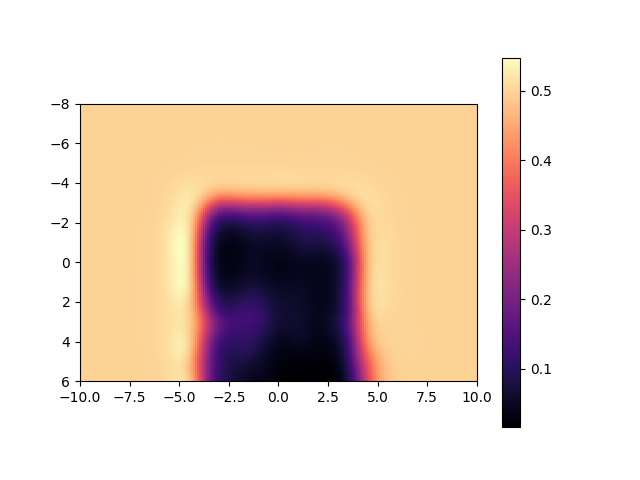
\includegraphics[width=75mm,trim={0 14mm 0
    10mm},clip]{Chap4/fig/ten_x_-1}}}%
    \hfill \subfloat[Plane
    $z=-2$]{{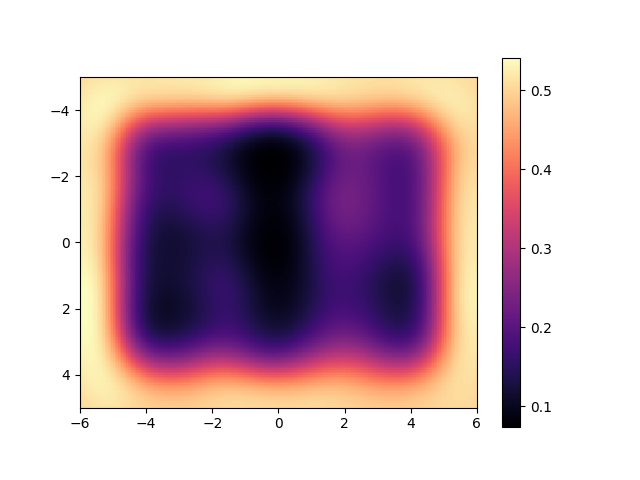
\includegraphics[width=75mm,trim={0 14mm 0
    10mm},clip]{Chap4/fig/ten_z_-2}}}%
    \\%
    \subfloat[Plane
    $x=0$]{{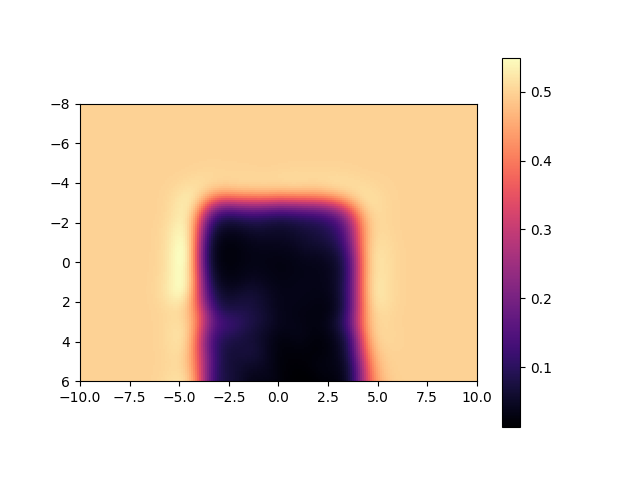
\includegraphics[width=75mm,trim={0 14mm 0
    10mm},clip]{Chap4/fig/ten_x_0}}}%
    \hfill \subfloat[Plane
    $z=-1$]{{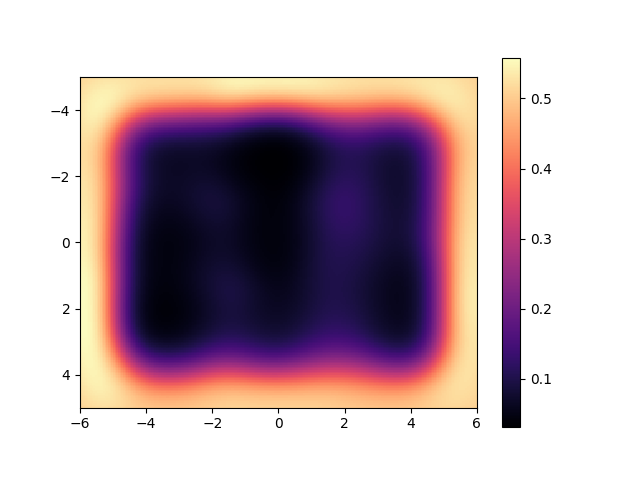
\includegraphics[width=75mm,trim={0 14mm 0
    10mm},clip]{Chap4/fig/ten_z_-1}}}%
    \\%
    \subfloat[Plane
    $x=1$]{{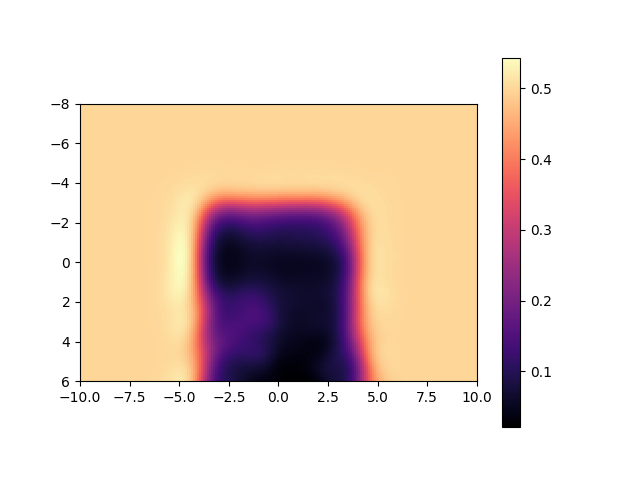
\includegraphics[width=75mm,trim={0 14mm 0
    10mm},clip]{Chap4/fig/ten_x_1}}}%
    \hfill \subfloat[Plane
    $z=0$]{{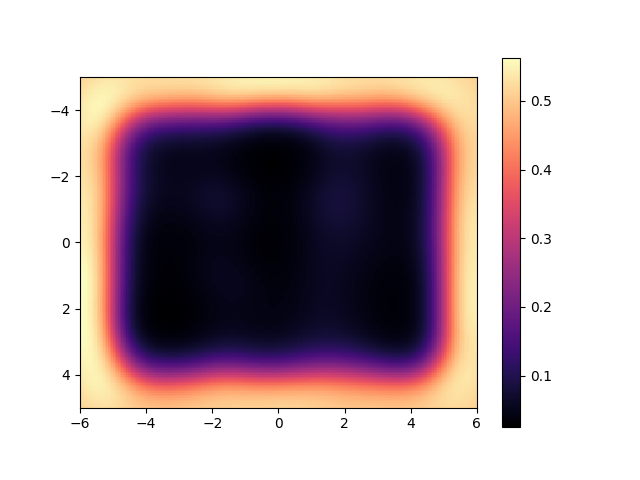
\includegraphics[width=75mm,trim={0 14mm 0
    10mm},clip]{Chap4/fig/ten_z_0}}}%
    \caption{Mapping with $10\%$ of available beams.}%
    \label{fig:ten_map}%
\end{figure}

\begin{figure}[ht]
    \centering
    \subfloat[Plane
    $x=-1$]{{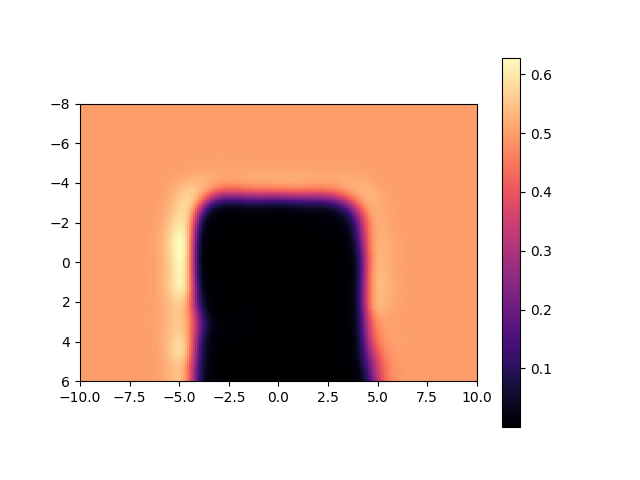
\includegraphics[width=75mm,trim={0 14mm 0
    10mm},clip]{Chap4/fig/thir_x_-1}}}%
    \hfill \subfloat[Plane
    $z=-2$]{{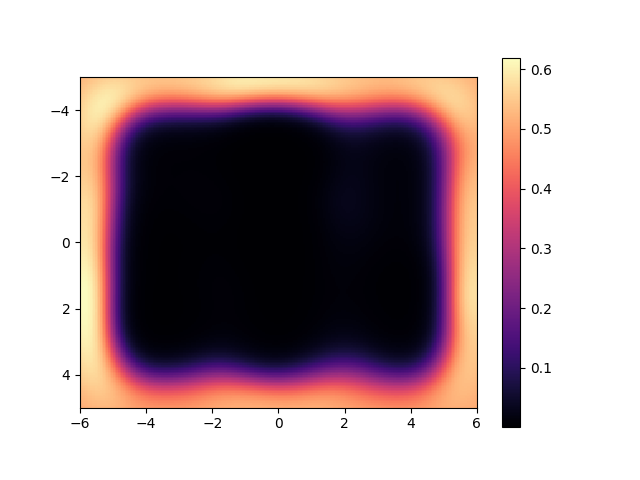
\includegraphics[width=75mm,trim={0 14mm 0
    10mm},clip]{Chap4/fig/thir_z_-2}}}%
    \\%
    \subfloat[Plane
    $x=0$]{{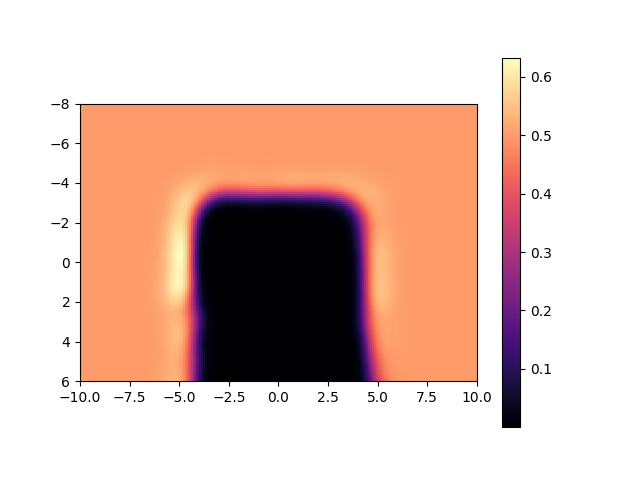
\includegraphics[width=75mm,trim={0 14mm 0
    10mm},clip]{Chap4/fig/thir_x_0}}}%
    \hfill \subfloat[Plane
    $z=-1$]{{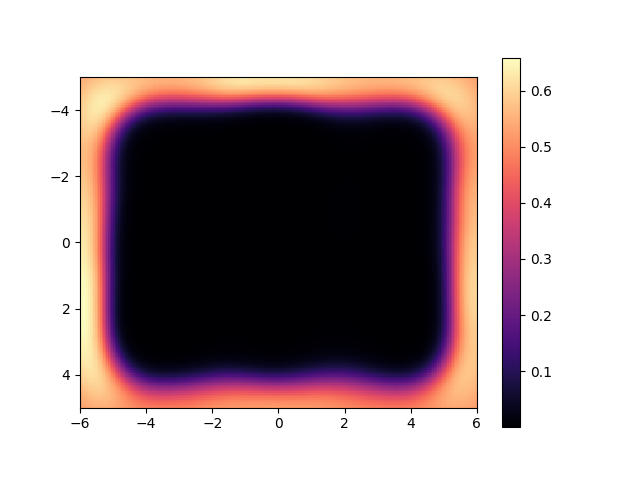
\includegraphics[width=75mm,trim={0 14mm 0
    10mm},clip]{Chap4/fig/thir_z_-1}}}%
    \\%
    \subfloat[Plane
    $x=1$]{{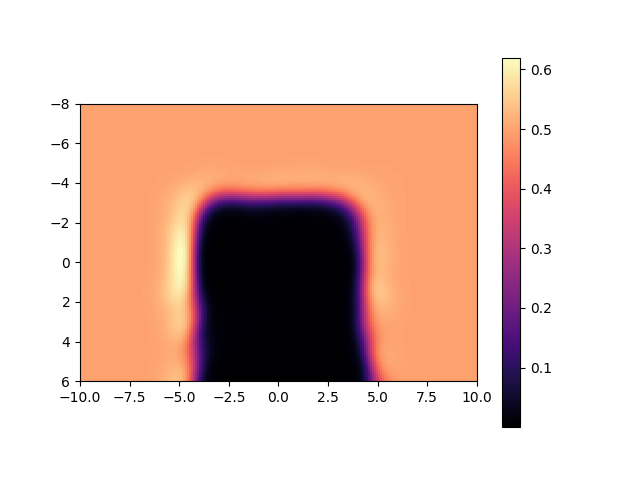
\includegraphics[width=75mm,trim={0 14mm 0
    10mm},clip]{Chap4/fig/thir_x_1}}}%
    \hfill \subfloat[Plane
    $z=0$]{{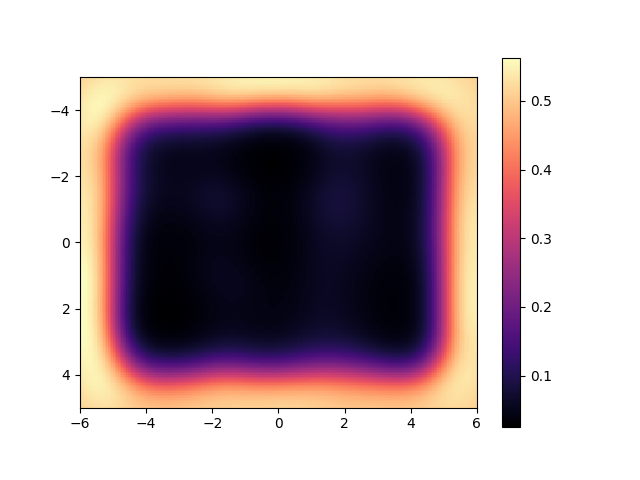
\includegraphics[width=75mm,trim={0 14mm 0
    10mm},clip]{Chap4/fig/ten_z_0}}}%
    \caption{Mapping with $30\%$ of available beams.}%
    \label{fig:thir_map}%
\end{figure}

\begin{figure}[ht]
    \centering
    \subfloat[Plane
    $x=-1$]{{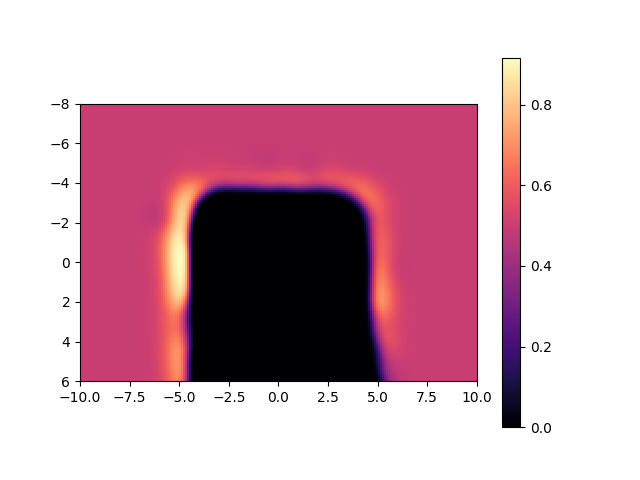
\includegraphics[width=75mm,trim={0 14mm 0
    10mm},clip]{Chap4/fig/full_x_-1}}}%
    \hfill \subfloat[Plane
    $z=-2$]{{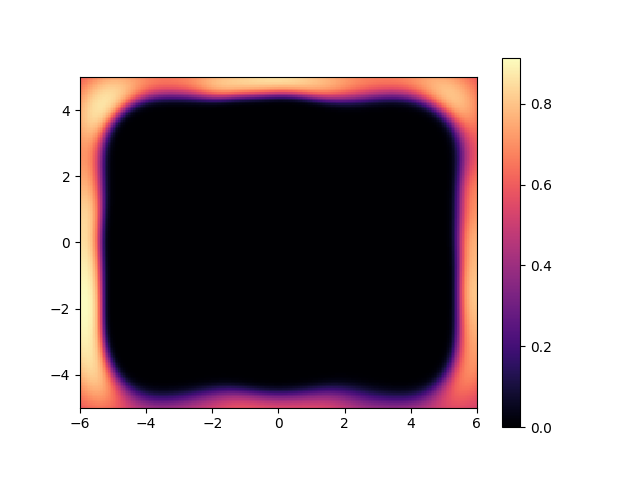
\includegraphics[width=75mm,trim={0 14mm 0
    10mm},clip]{Chap4/fig/full_z_-2}}}%
    \\%
    \subfloat[Plane
    $x=0$]{{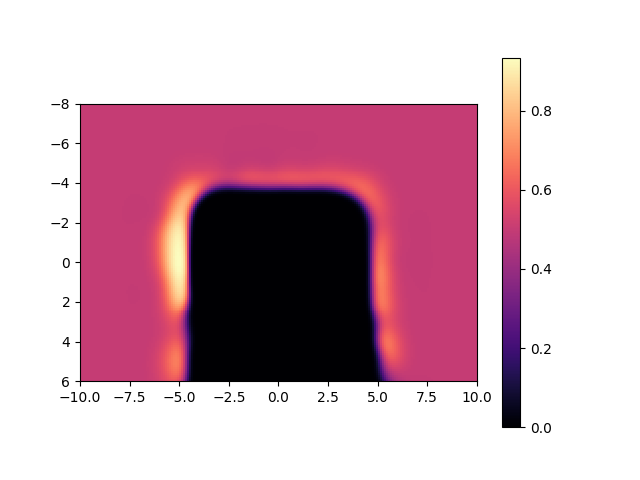
\includegraphics[width=75mm,trim={0 14mm 0
    10mm},clip]{Chap4/fig/full_x_0}}}%
    \hfill \subfloat[Plane
    $z=-1$]{{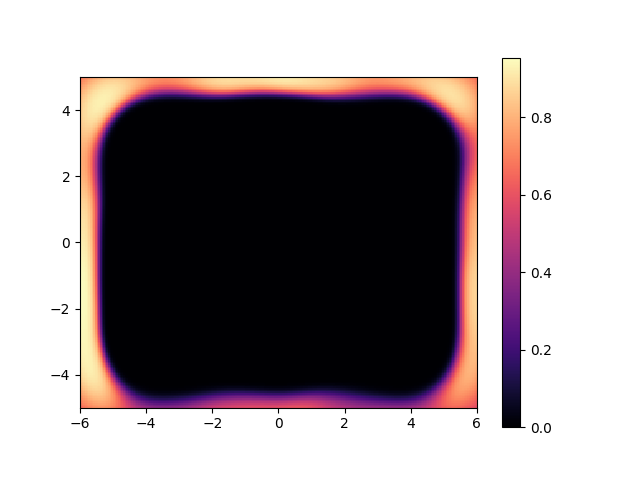
\includegraphics[width=75mm,trim={0 14mm 0
    10mm},clip]{Chap4/fig/full_z_-1}}}%
    \\%
    \subfloat[Plane
    $x=1$]{{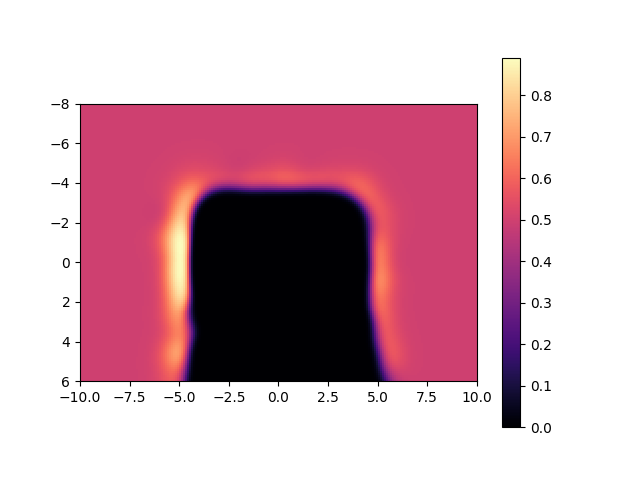
\includegraphics[width=75mm,trim={0 14mm 0
    10mm},clip]{Chap4/fig/full_x_1}}}%
    \hfill \subfloat[Plane
    $z=0$]{{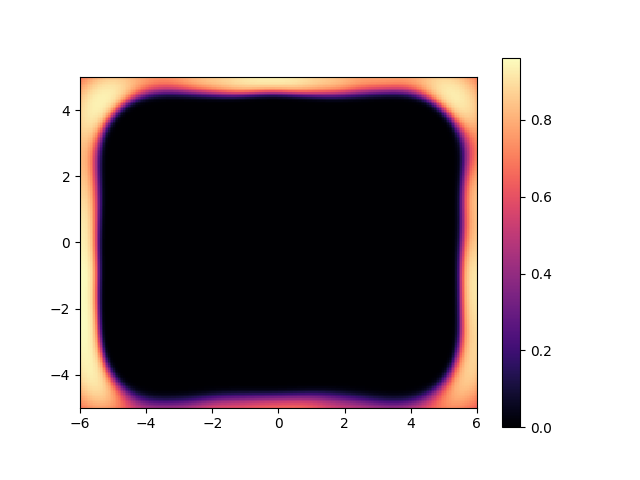
\includegraphics[width=75mm,trim={0 14mm 0
    10mm},clip]{Chap4/fig/full_z_0}}}%
    \caption{Mapping with $100\%$ of available beams.}%
    \label{fig:full_map}%
\end{figure}



% Directional Processing of
% Ultrasonic Arc Maps and
% its Comparison with
% Existing Techniques - Pe and Po com occupancy grid